\documentclass[conference]{IEEEtran}
\IEEEoverridecommandlockouts
% The preceding line is only needed to identify funding in the first footnote. If that is unneeded, please comment it out.
\usepackage{cite}
\usepackage{amsmath,amssymb,amsfonts}
\usepackage{algorithmic}
\usepackage{graphicx}
\usepackage{textcomp}
\usepackage{xcolor}
\def\BibTeX{{\rm B\kern-.05em{\sc i\kern-.025em b}\kern-.08em
    T\kern-.1667em\lower.7ex\hbox{E}\kern-.125emX}}
\begin{document}
\begin{titlepage}

\title{Sharing and Binding for General Circuits\\}

\author{\IEEEauthorblockN{Benedikt Lipinski}
\IEEEauthorblockA{\textit{Interaktionstechnik und Design)} \\
\textit{Hochschule Hamm Lippstadt}\\
Lippstadt, Germany \\
benedikt.lipinski@stud.hshl.de}
}
\maketitle
\begin{abstract}

\end{abstract}
\end{titlepage}
\begin{titlepage}
\tableofcontents
\end{titlepage}


\newpage
\section{Introduction}
Durch das menschliche verlangen Problemstellungen zu-gunsten schwindender Komplexität und erhöhtem Komfort zu automatisieren und zu brechen, wurden genau diese Anforderungen auf die elektrischer Schaltungen umgelegt. 
\subsection{Problemstellung}
Nicht erst durch Moderne Entwicklungen, wie digitale Vernetzung mit dem Internet der dinge  oder das Autonome Fahren wird die Betrachtung,  Zeitliche und Finanzielle Aspekte für die entwicklung multidimensionaler Systeme notwendig. Allerdings lassen genau diese Entwicklungen, die Komplexität sprunghaft ansteigen.

\subsection{Logische Bausteine}
Realisierbar werden elektrische Verschaltungen in der Digitaltechnik erst durch den einsatz sogenannter Logikbausteine, die mit einander kombiniert ein vorher genau bestimmtes verhalten der geplanten Schaltung verursachen.
Hierbei übernehmen verschiedene Bausteine verschiedene Aufgaben, die mal weniger und mal mehr kompliziertere Operationen beinhalten. 
\subsubsection{AND-Gatter}
Eine der Grundoperationen, die in fast jeder schaltung zu finden ist, ist die AND zu deutsch die UND Operation. hierbei wird der eingang erst auf logisch 1 geschaltet, wenn alle eingänge dies ebenfalls sind.\\
\begin{tabular}[h]{ccc}
x&y&Out\\
0&0&0\\
0&1&0\\
1&0&0\\
1&1&1\\
\end{tabular}
\subsubsection{OR-Gatter}
Das Ergebnis des OR-Gatters ist in dem Fall Wahr, wenn einer seiner Eingänge Wahr ist.\\
\begin{tabular}[h]{ccc}
x&y&Out\\
0&0&0\\
0&1&1\\
1&0&1\\
1&1&1\\
\end{tabular}
\\Simple Schaltungen lassen sich durch das gezielte aneinanderreihen von AND und OR Gattern gut realisieren, sollte aber 
\subsubsection{Multiplexer}
Multiplexer werden benutzt, wenn eine Parallele Verarbeitung aus unterschiedlichsten gründen nicht möglich ist, das kann zum einen eine nicht ausreichende Verfügbarkeit an Kanälen sein, aber auch eine bewusste Entscheidung weniger Kanäle aus kosten gründen zu benutzen sein. Dieser schritt kann gewählt werden, wenn Verläufe zwar parallel laufen aber nur exklusiv ausgeführt werden, das bedeutet, dass nach einer elementaren Entscheidung nur einer der beiden Stränge ausgeführt werden kann. Beeindruckend allerdings ist, das Multiplexer trotz ihrer fortgeschrittenen eignenschaften gegenüber den Grundbausteinen, doch recht simple aus genau diesem erzeugt werden kann. So ergibt sich für einen Einfachen Multiplexer das schaltbild aus 2 AND-Gattern, Einem NOT- Gatter und einem OR- Gatter. .....
\subsubsection{FPGA}
Der Einsatz von diesen Grundelementen ist für das erreichen des Ziels völlig hinreichend, doch benötigt sie eine sehr hohe fläche, auf der sie Verbaut werden muss. Ein zu erreichendes Ziel ist, die Fläche auf der die schaltung realisiert werden muss zu verringern. Dies ist durch die verwendung von halbleitern und die entwicklung von Integrierten schaltkreisen auch erfolgreich gelungen, allerdings besitzen diese sogenannten IC's den nachteil, das ihre Schaltung wie die einer realisierung mit Bausteinen auch fest gebunden ist. Ein Nachteil, den FPGA (Field Programmable Gate ARRAY) Bauteile nicht besitzen, ihr Vorteil ist die Zusammensetzung aus Zusammengeschalteten Baugruppen aus Logikbausteinen, FlipFlops und derer verbindung mit Multiplexern. In FPGA's kann das Verhalten der Eingänge zu den Ausgängen über{\color{red}...... }"Programmiert" werden.
\subsection{Strategien zur Architektur Optimierung}
Mit steigender Komplexität der verschaltungen steigt zwingend auch die anzahl der  zu nutzenden Bauteile, zudem steigt auch die verwendung performaterer Bausteine stetig um die abarbeitung bezüglich leistung und aller zeitlicher deadlines einhalten zu können. Nachteilig ist vor dem hintergrund ebenfall, dass Bausteine mit einer höhreren leistung, oftmals auch eine erhöhten platzbedarf einfordern\cite[S.327]{2}.\\
Ziel ist es, strategien Umzusetzen, die,  die Chipfläche verringern, ohne dabei die Lesitungsfähigkeit der Schaltung zu beeinflussen. Leider ist dieses Problem nicht mit der einhaltung beider anforderungen zu vereinbaren, wodurch zum Beispiel die verminderung der kosten durch senkung der chip Anzahl und Fläche immer auch zum nachteil der Performance agiert.Der zusammenhang zwischen Fläche und der erzeugten leistungsverminderung ergibt sich aus der Fläche $a$ in der Einheit Gatteräquivalent $(Gate Equivalent GE)$ das die größe des Simplesten gatters wiederspiegelt\cite[S.326]{2} und der Performance die den kehrwert der Ausführungszeit $T_{ges}$ wiederspiegelt $\frac{1}{T_{ges}}$, die sich wieder aus der Takzeit $T_c$ multipliziert mit der Latenz $\lambda$ zusammensetzt
\cite[S.325-326]{2}.\\
 Eine Mögliche Realisierung der schaltung mit einer bestimmten Performance, bei einer Bestimmten Fläche lässt sich als punkt in einem diagramm darstellen,dessen achsen sowohl die Chipfläche, die Latenz und den Takt abbilden\cite[S.326]{2}.
 Dieses vorgehen\cite{?} ist in diesem fall notwendig, da mehr als eine Variable optimiert werden muss, und es dementsprechend mehr als eine gültige lösung dieses Problems gibt. Als mögliches Hilfsmittel kann hier die Pareto-optimierung verwendet werden. Die Pareto-Optimierung erzeugt eine Kompromisslösung durch die Gewichtung jeder einzelfunktion. Die Idee dahinter ist, dass die Gewichtung die Wichtigkeit der Einzelfunktion repräsentiert und ihr bei steigendem gewichti mehr aufmerksamkeit verleit\cite[S.45]{4}



\subsection{Allocation}

%...ist eigl. Binding wird aber auch mit der betrachtung der zur verfügung stehenden Resourcen in verbinduggebracht 

%MEnge der zur Verfügung stehenden recourcen 
%Die Allokation ist eine Funktion, die angibt zu welchem Ressourcen typ Wiviele REssourcen zu r verfügung stehen 




Nicht nur, aber vor allem aus Kosten und Platzgründen stehen der Entwicklung selten unbegrenzte resourcen zur verfügung. Aus diesem Grund kann die Betrachtung der zur verfügung stehenden resourcen zwingend notwendig werden. Somit ist das ergebnis der allokierung nach Teich \cite{1}    
, eine funktion $ \alpha(r_k)$ die angibt wie viele verfügbare Bauteile es zu einer Jeweiligen Resourcentyp gibt.\\
Damit würde, wenn vom Resourcentyp Mulitplizier: $r_1$,Beispielweise 1 Einheiten zur verfügung stehen die Allokierungsfunkion $\alpha(r_1) = 2$ lauten. Die Funktion der Allokation zeigt deshalb ziemlich genau welche probleme beziehungsweise zeitliche veränderungen entstehen durch die grenzen, die durch die begrenzte verfügbarkeit an Resourcen gegeben werden. Dies kann ein nützlicher zwischenschritt sein um den überblick zu behalten,den Teich mittels eines Ressourcen graphen anschaulich darstellt.In vielen Literaturen allerdings wird dieser schritt auch in die Bindung integriert und nicht extra behaldelt.
\subsection{Binding}
Im unterschied zur Allokierung wird in der Bindung schließlich festgelegt welche Resource welche operation zugeteilt bekommt,also die Zuweisung von Operationen zu bestimmten hardware Komponenten \cite{3}. in einer Utopischen vorstellung in der Kosten und Fläche keine rolle spielen würden, könnte für jeden Rechnenschritt, jede Operation, also zum beispiel für jede Multiplikation oder jeden vergleich eine eigene Komponete Benutzt werden. Leider ist diese vorstellung in der Praxis nicht durchführbar,  da jedes gesparte bauteil auf eine Große stückzahl gerechnet den Kostendruck lindert.Das ist zudem auch nicht zwingend nötig, da Beilspielsweise ein Vergleich nach eine Addition, welche beide durch eine Alu realisiert werden können, nicht unbedingt durch 2 verschiedene Hardware einheiten umgesetzt werden müssen, da der vergleich erst stattfinden kann wenn das ergebnis der Addition vorliegt. genannt wird dies in diesem fall ein Optimal Resource sharing oder zu Deutsch ein Optimales ausnutzen einer Resource\cite{2}.\\
Die Bindung bietet ein Tool, das veranschaulicht wie optimal die vorhandene schaltung auf und mit den gegebenen Bauteilen realisiert wird. Da das engültige Ziel eine Optimale ausnutzung der vorhandenen resourcen ist müssen nun schrittweise die benötigten Bauteile minimiert werden, dies wird erreicht indem anfangs jede Operation einem bauteil zugeordnet wird, es wird ein sogenannte dedizierte Ressource erzeugt, ein spezialfall \cite[S. 150]{3} 
\begin{figure}[h]
\center{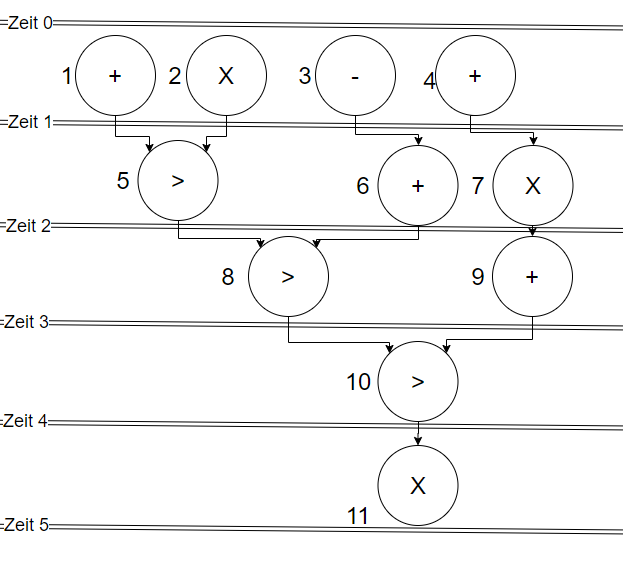
\includegraphics[scale=0.55]{fig_bsp_binding}}
\caption{Besipiel zur Bindung}
\label{fig.1}
\end{figure} 

Dem Bild ist zu entnehmen das in diesem beispiel für die zuordnung jeder Aufgabe zu einer Resource:11 Bauteile benötigt werden.
 Die sich aus 3 Multiplikationen = $r_1$ und aus 8 operationen für eine Arithmetisch logisch einheit $r_2$ ergibt.\\
\begin{tabular}[h]{ccc}
$v_i$&$\beta(v_i)$&$\gamma(v_i)$\\
$v_1$&$r_2$&1\\
$v_2$&$r_1$&1\\
$v_3$&$r_2$&2\\
$v_4$&$r_2$&3\\
$v_5$&$r_2$&4\\
$v_6$&$r_2$&5\\
$v_7$&$r_1$&2\\
$v_8$&$r_2$&6\\
$v_9$&$r_2$&7\\
$v_10$&$r_2$&8\\
$v_11$&$r_1$&3\\
\end{tabular}
Da es sich, um ein recht einfach zu überblickendes beispiel handelt, lässt sich durch einen geübten blick bereits erkennen wie eine Optimierung aussehen könnte. Im ersten Zeitslot ist abzulesen, das 3 Arithmetische operationen und eine Multiplikation durchgeführt werden, somit werden 3 ALU Einheiten und ein Multiplizierer benötigt.Im weiteren verlauf lässt sich unteranderem erkennen das in keinem weiteren zeitzlot mehr als 3 ALU einheiten gebraucht werden, deswegen ist dies auch unsere minimal benötigte anzahl an Resourcen dieses typs. Ganz genau deutlich wird dies durch eine veranschaulichung in einer tabelle.
\begin{tabular}[h]{ccc}
Zeitslot&ALU&Multiplizierer\\
1&3&1\\
2&2&1\\
3&2&0\\
4&1&0\\
5&0&0\\
\end{tabular}
\\Aus der Tabelle kann nun abgelesen werden, das 3 Resourcen des Typs ALU benötigt werden und 1 des Typs Mulitplizierer.\\
Übertragen auf die obere Tabelle ensteht nun folgendes Binding.\\
\begin{tabular}[h]{ccc}
$v_i$&$\beta(v_i)$&$\gamma(v_i)$\\
$v_1$&$r_2$&1\\
$v_2$&$r_1$&1\\
$v_3$&$r_2$&2\\
$v_4$&$r_2$&3\\
$v_5$&$r_2$&1\\
$v_6$&$r_2$&2\\
$v_7$&$r_1$&1\\
$v_8$&$r_2$&1\\
$v_9$&$r_2$&2\\
$v_10$&$r_2$&1\\
$v_11$&$r_1$&1\\
\end{tabular}
Somit wurden in diesem beispiel 5 Alu einheiten die einen anteil von $62,5\%$ ausmachen eingespart. Bei den Multiplizierern wurde die benötigten Resourcen auf $\frac{1}{3}$ reduziert.

%-Welche INstanz und welcher Ressourcentyp
%-connected die ressourcen und instanzen zu eioner bestimmten aufgabe 

\subsection{Sharing}
das sharing beschreibt zusammen mit dem Binding,  die effektive mehrfachnutzung der Ressourcen, welches der minimierung der verwendeten hardware dient und somit zu reduzierung von Flächen und kosten problemen beiträgt. wobei das ziel des Sharing die frage nach dem Alghoritmus zur optimerung ist und anschließend mit einem Binding endet. In dem Kapitel Binding wurde ein einfach im Kopf zu lösendes Beispiel gezeigt, leider bleibt es in der Realität nicht immer bei so einfach zu lösenden systemen, so dass da schnell der überblick verloren gehen kann und zudem ein system unter umständen nicht zu lösen wäre. Aus diesem grund befasst sich dass sharing mit der frage wie ein vorhandenes system effektiv optimiert werden kann.Zu den Verwendeten Alghoritmen zählen unter anderem aus dem breich der REsource Dominated Circuits das Register sharing, Multiport Memory Binding und das Bus sharing and Binding und für den bereich der general circuits, sind es Unconstrained minimum - Area Binding, Performance Constrained Binding und zu letzt Performance Directed Binding.   
\section{Grundlegendes}

\subsection{Kompatiblitäts- und Konfliktgraphen}
Als vorrausetzung, um überhaupt eine sinnvolle Bindung beziehungsweise Allokierung erzeugen zu können muss sich im 1. schritt einmal mit dem eigentlichen problem befasst werden. Um das Problem darstellen zu können wird ein Graph aufgestellt, der die eigenschaften der elemente beschreibt. Dieser Schritt ermöglicht die betrachtung der einzelnen operationen mit einander und stellt auf welche mit einander Kompatibel sind und welche ein kritisches verhalten zu einander aufweisen.\\
Zwei oder mehr Operationen sind mit einander Kompatibel und können an die Gleiche Resource gebunden werden wenn sie nicht mit einander Konkurrieren und wenn sie dem gleichen Resourcen-typen angehören\cite[S.231]{3}\\
Das bedeutet konkreit, dass aufgaben mit einander kompatibel sind, wenn sie nicht im gleichen Zeitslot neben einander anliegen und wenn sie des gleichen typs sind zum Beispiel Addierer.
Die entwicklung der ges graphensystems kann grundsätzlich über 2 ansätze erfolgen, zum einen kann ein Kompatiblitätsgraph oder Verträglichkeitsgraph entwickelt werden, dieser graph gibt an welche Operationen verträglich zu einander sind und somit keine probleme darstellen komplemäntar dazu lässt sich durch den Konflikt graphen angeben welche Operationen im konflik zu einander stehen und eine genauere betrachtung bedüfen.\\
Ein Ressourcen Verträglichkeitsgraf ist definiert durch $ G_+(V,E)$ in denen die Knoten durch $ V = \{v_i;i=1,2,...,n\}$ definiert werden und die Kanten durch $E = \{\{v_i,v_j\}i,j = 1,2,...,n\}$ Die Knoten stellen die Operationen an sich dar, wohingegen die Kanten die Kompatiblen Operationspaare angeben\cite[S.231]{3}.\\
Zusammen gefasst nach  Teich \cite[S. 181-182]{1} lassen sich folgende verträglichkeiten für den kompatiblitätsgraphen aufführen:\\

demnach ist eine \textbf{Schwache verträglichkeit} gegeben, wenn zwei knoten des Graphen
eines Grahen mit einander verbunden sind und des gleichen Types angehören also zum beispiel eine Addition und ein Vergleich, da beide durch eine Arithmetisch logische einheit Verarbeitet werden können.\cite{?}\\

\textbf{Ablaufplan verträglich} ist ein graph hingegen, wenn seine Knoten als erste bedingung vom gleichen typ sind, also wie bei der schwachen verträglichkeit zum Beispiel aus 2 operationen vom typ Multiplizierer. Zum zweoten muss die bediingung erfüllt sein, das die starzeit des ersten knoten vor der des zweiten knotens liegen muss. Das bedeutet, dass Knoten die Ablaufverträglich sind nicht in dem selben zeitslot ausgeführt werden dürfen, andernfalls wären sie nicht Ablaufplan vertträglich\cite{?}.\\

Als leztztes definiert sich die \textbf{Starke verträglichkeit}, durch zwei Knoten die wieder vom gleichen typ sind und zudem von einandern abhängig sind. Das bedeutet die beiden knoten sind in einem logischen strang durch einen pfad im ablaufplan mit einander verbunden.\cite{?}

Die Graphische umsetzunge des Verträglichkeitsgraphes mit dem Beispiel aus den vorherigen kapiteln sieht dann wie folgt aus: 
\begin{figure}[h]
\center{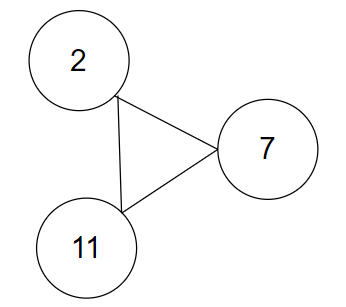
\includegraphics[scale=0.55]{fig_comp_mult}}
\caption{Verträglichkeitsgraph Mulitplizierer}
\label{fig.2}
\end{figure}\\
Aus den vorherigen kapiteln, wissen wir bereits, dass für die Optimierung der verschaltung nur ein Multiplizierer benötigt wird und genau das können wir in diesem beispil nun auch grafisch betrachten. Zu sehen ist, dass jeder knoten mit einer kante verbunden ist und somit sind alle Operationen mit einander Ablaufplan verträglich, weswegen der einsatz von nur einem Multiplizierer nun auch Optisch besser nachzuvollziehen ist.\\
\begin{figure}[h]
\center{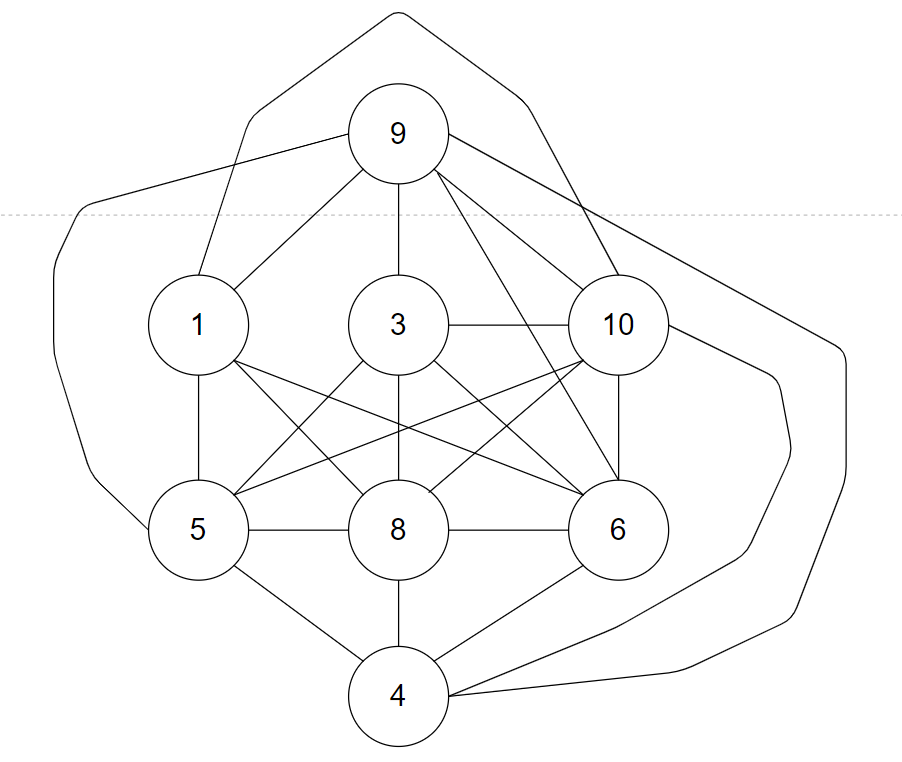
\includegraphics[scale=0.55]{fig_comp_alu}}
\caption{Verträglichkeitsgraph Arithmetisch logische einheit mit Cliquen}
\label{fig.4}
\end{figure}
Als nächsten schritt werden nun sogenannte Cliquen eingezeichnet, sie repräsentieren die zusammenfassung Mehrerer Operationen und zeigen ihre zusammenführung auf eine Komponente, so das für jede clique genau eine Komponente eingesetzt wird. Zu sehen ist, das Bei dem Verträglichkeitsgraphen der Mulitplizierer genau eine Clique eingezeichnet werden muss. Da mit steigender Komplexität der aufgabe, auch die Komplexität für das einzeichen der Cliquen steigt, bietet sich dieses verfahren leider nur für die anwendung an simple verschaltungen an, der Grund hierfür ist die klassifizierung dieses problems als NP-Hartes Problem.\cite[S.361]{2}\\
\begin{figure}[h]
\center{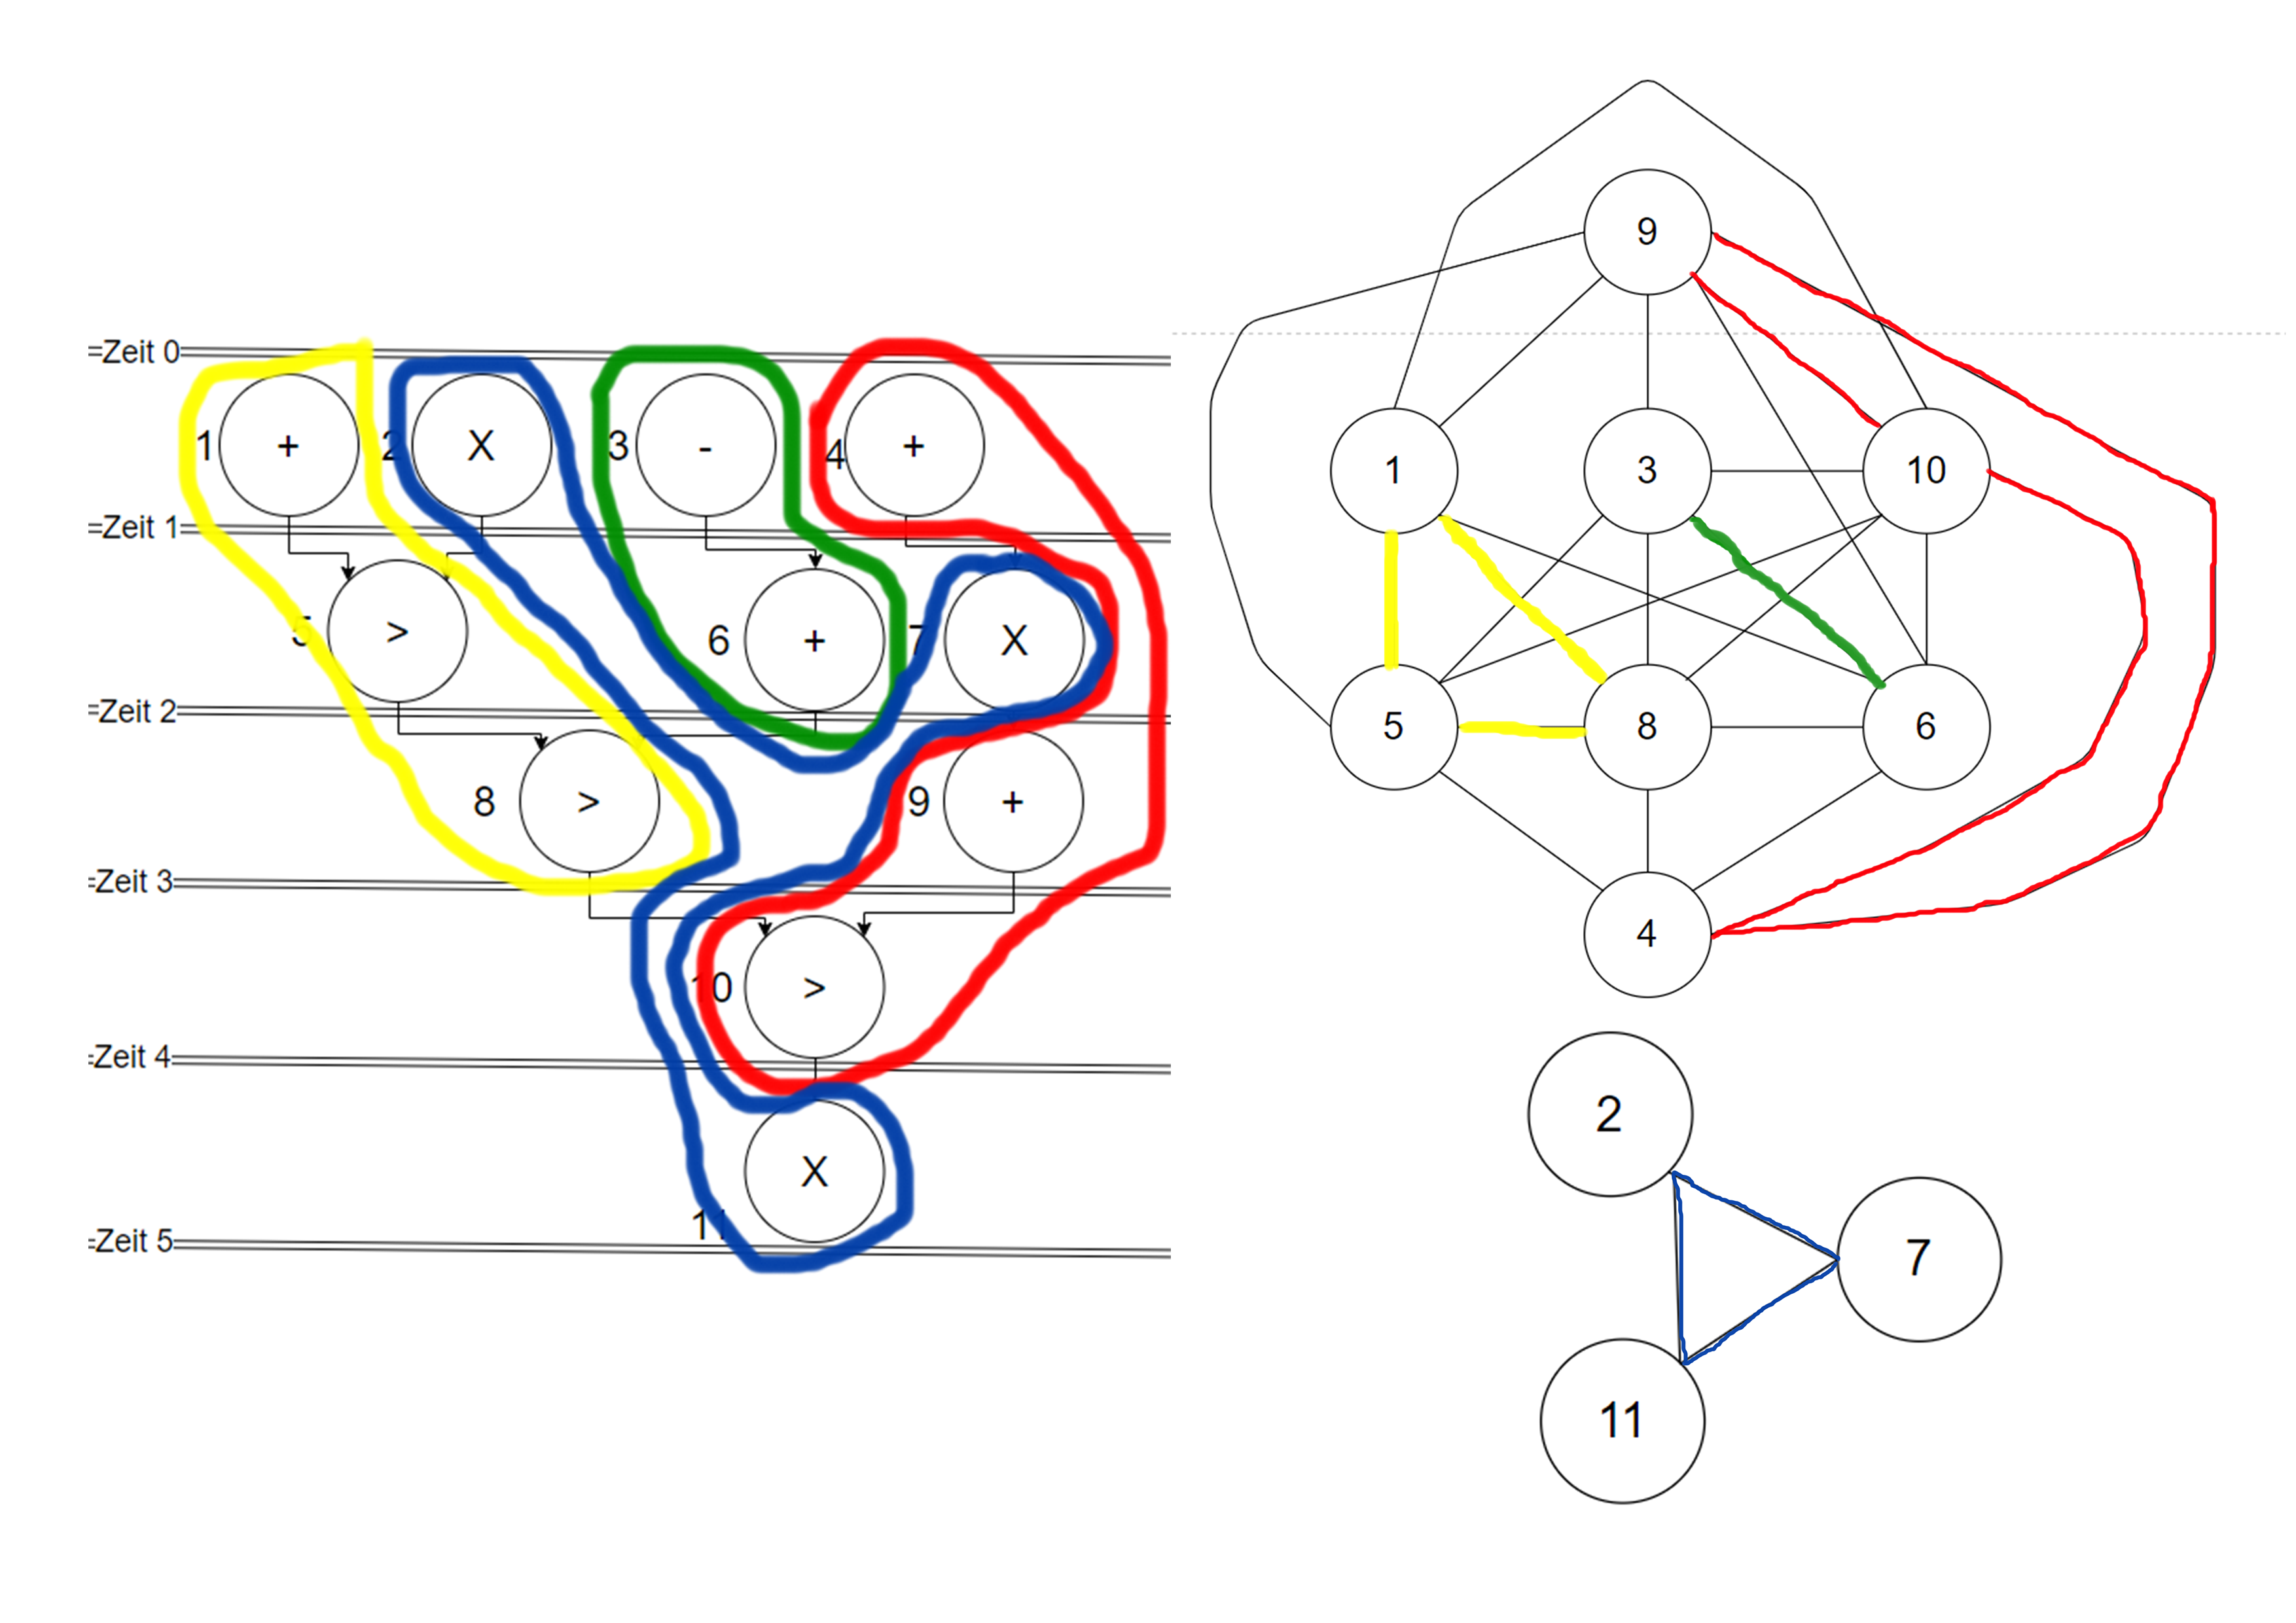
\includegraphics[scale=0.08]{fig_cliquen}}
\caption{Ablaufplan und verträglichkeitsgraphen mit Cliquenbildung}
\label{fig.3}
\end{figure}

%Graph zur betrachtung der Verträglichkeit einzelner Operationen
%zeigt auf einen bliock welche operationen mit einander kombiniert werden können %und welche nach folgenden regeln auf keinen fall kombiniert werden können

%-Schwach verträglich
%wenn vom gleichen ressourcentyp ?? 
%-Ablaufplan verträglich
%alternativ sind
%-Stark verträglich
%nicht gleichzeitig sind und mit einem gerichteten graph verbunden 




\subsection{Resource Dominated circuits}
da probleme leider ein wenig komplizierter 

behamndelt wir die grundlegende optimierung mit dem grundlagen wissen aus Konflikt und Optimum graph 

z.b mittels register sharing
-G.micheli S 156 
\section{General Circuits}
\subsection{Allgm.}

ganz allgemein wird jetzt auch die verzögerung durch steuerlogik und die verkabeluing betrachtet, also wie man so schön sagt ein reale verschaltung
\subsection{Baugruppen}
 \subsubsection{Register}
 \subsubsection{Steuerlogik}
 \subsubsection{Verkabelung}
 \subsubsection{kontroll einheiten}
\section{Sharing and Binding for General Circuits}
\subsection{Unconstrained minimum - Area Binding}
\subsection{Performance Constrained Binding}
\subsection{Performance Directed Binding}
\section{Gleichnis,vorgestellter Algorithmen}
\section{Ausblick}

\begin{thebibliography}{00}
\bibitem{1} Jürgen Teich, Christian Haubelt, Digitale Hardware/Software-Systeme, Synthese und Optimierung, 2. Auflage,Springer,2007
\bibitem{2} Dr.Walter Lange, Prof.Dr.Martin Bogdan, Entwurf und Syntese von Eingebetteten Systhemen, Ein Lehrbuch,Oldenbourg Verlag München, 2013
\bibitem{3} DEMICH
\bibitem{4} Martin Pieper, Mathematische Optimierung, Eine Einführung in die Kontinuierliche Optimierung mit Beispielen,Springer Spektrum,2017
\end{thebibliography}
\vspace{12pt}


\end{document}
